\chapter{Experiments}\label{ch:experiments}

This chapter presents simulation scenarios chosen to demonstrate the performance and limitations of the simulator, as well show the concept of OAL.

A common configuration for all experiments is given in Table \ref{tab:var-allcases}. The individual configurations are presented in the respective sections.

\begin{table}
\centering
    \begin{tabular}{|c|c|c|}
        \hline
         \textbf{Description} & \textbf{Variable name} & \textbf{Value} \\
         \hline \hline
         Link length $[m]$& \texttt{l} & $1$ \\
         \hline
         Link mass $[kg]$& \texttt{m} & $1$ \\
         \hline
         Obstacle safety radius $[m]$& \texttt{obstacle\char`_radius} & $0.1$\\
         \hline
    \end{tabular}
    \caption{Common simulation configuration for all cases}
    \label{tab:var-allcases}
\end{table}



%---------------------------------------------------------------------------------------
%---------------------------------------------------------------------------------------
%---------------------------------------------------------------------------------------

\section{Obstacle-free environment}

This section demonstrates how the robot behaves without the influence of obstacles in the environment. Special emphasis is placed on the the path alignment performance. 

\subsection{Single reference computed torque control}\label{subseq:case11}

This experiment is to demonstrate the two different damping modes of the computed torque controller applied in the rest of the experiments. For simplicity, a static setpoint scenario is chosen. The variable configuration for the experiment is summarized in Table \ref{tab:var-case-1-1}.

\begin{table}[H]
\centering
    \begin{tabular}{|c|c|c|}
        \hline
         \textbf{Description} & \textbf{Variable name} & \textbf{Value} \\
         \hline \hline
         Simulation time $[s]$& \texttt{simTime} & $30$ \\
         \hline
         Simulation sample time $[s]$& \texttt{h} & $0.01$ \\
         \hline
         Number of links & \texttt{n} & $4$ \\
         \hline
         Joint angle setpoints $[rad]$ & \texttt{q\char`_ref} & $[0, \pi/2, -\pi/3, -\pi/2]$ \\
         \hline
         Initial joint angles $[rad]$ & \texttt{q\char`_0(1:n)} & $[0, 0, 0, 0]$ \\
         \hline
         Initial position $[m]$ & \texttt{q\char`_0(n+1:n+2)} & $[0, 0]$ \\
         \hline
    \end{tabular}
    \caption{Simulation configuration for \ref{subseq:case11}}
    \label{tab:var-case-1-1}
\end{table}


Figure \ref{fig:case1-1} shows the different damping-cases using the computed torque controller following joint angle references plotted with dashed lines. It should be noted that the joint angle $q_1 = \phi_1$ is not included as it is a virtual coordinate and not directly actuated.

\begin{figure}[H]
    \centering

    \subfloat[Critically damped]{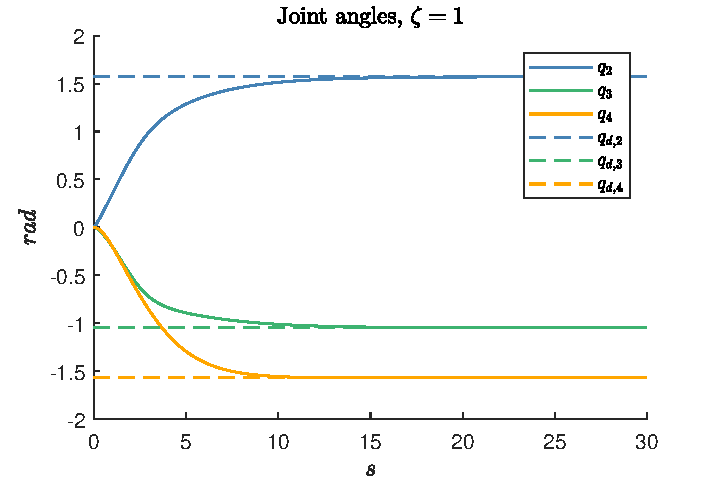
\includegraphics[totalheight=0.31\textheight]{figures/case-1-1/control-critdamped.pdf}}

    \subfloat[Overdamped]{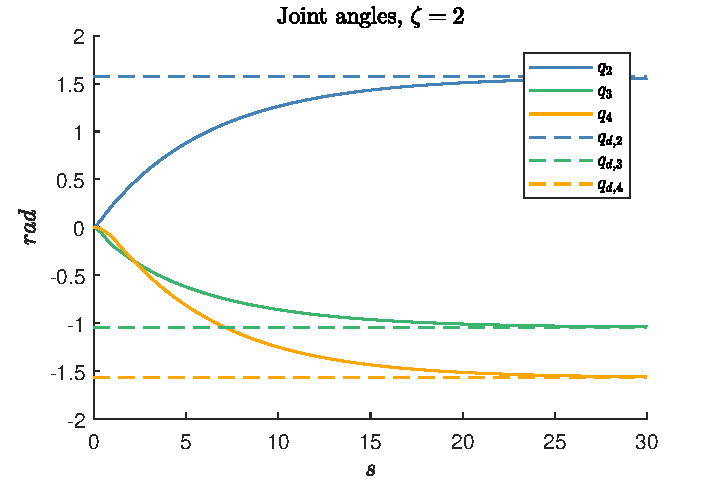
\includegraphics[totalheight=0.31\textheight]{figures/case-1-1/control-overdamped.pdf}}

    \caption{Simulation demo - computed torque control}
    \label{fig:case1-1}
\end{figure}

Because slow motions are desired to avoid abrupt movement, the overdamped configuration with $\zeta = 2$ is mainly used throughout the experiments. The underdamped case is not relevant for this project and thus left out.

The proportional gain is chosen to be $\mathbf{K_p} = 0.4 \mathbf{I}$ in all cases. The relation in (\ref{eq:control2}) with $\zeta=1$ and $\zeta=2$ yields $\mathbf{K_d} = 1.3 \mathbf{I}$ and $\mathbf{K_d} = 2.5 \mathbf{I}$ respectively.




%---------------------------------------------------------------------------------------
%---------------------------------------------------------------------------------------

\subsection{Path alignment}\label{subseq:case12}

In this case, the robot is initialized with two different start positions before attempting to adjust to the same path (\ref{eq:path}), which consists of line segments and quadrants. The start positions together with remaining variable configurations are summarized in Table \ref{tab:var-case-1-2}.

\begin{equation}\label{eq:path}
    y(x) =
    \begin{cases}
        0, & \text{if } x < 2.2 \\
        \sqrt{4 - (x - 2.2)^2} + 2, & \text{if } x \in [2.2, 4.2] \\
        -\sqrt{4 - (x - 6.2)^2} + 2, & \text{if } x \in [4.2, 6.2] \\
        -4, & \text{if } x > 6.2
    \end{cases}
\end{equation}

\begin{table}[H]
\centering
    \begin{tabular}{|c|c|c|}
        \hline
         \textbf{Description} & \textbf{Variable name} & \textbf{Value} \\
         \hline \hline
         Simulation time $[s]$& \texttt{simTime} & $10$ \\
         \hline
         Simulation sample time $[s]$& \texttt{h} & $0.001$ \\
         \hline
         Damping ratio & \texttt{zeta} & $2$ \\
         \hline
         Number of links & \texttt{n} & $4$ \\
         \hline
         Joint angle setpoints $[rad]$ & \texttt{q\char`_ref} & \makecell{Given by the path \\projection method} \\
         \hline
         Initial joint angles $[rad]$ & \texttt{q\char`_0(1:n)} & $[0, 0, 0, 0]$ \\
         \hline
         Initial position $[m]$ & \texttt{q\char`_0(n+1:n+2)} & $[0, 0]$ \\
         \hline
         \makecell{Initial position part 1 $[m]$\\Initial position part 2 $[m]$} & \texttt{q\char`_0(n+1:n+2)} & \makecell{$[0, 0]$ \\ $[0, 1]$} \\
         \hline
    \end{tabular}
    \caption{Simulation configuration for \ref{subseq:case12}}
    \label{tab:var-case-1-2}
\end{table}

The Figures \ref{fig:case1-2a} and \ref{fig:case1-2b} show the start and end position of the adjustment in a 15 second interval. The dashed lines are connections between the joints and their respective projected points on the path. The lines for the first two joints are displayed in gray because they are disregarded in the computation of the reference angles. The path projection method simply regards endpoints of controllable links. Furthermore, the method is not considering that the snake robot should be stretched out along the path at all times. A repercussion of this will become clear in the experiment in \ref{subseq:case24}.

\begin{figure}[H]
    \centering
    
    \subfloat[$t = 0 s$]{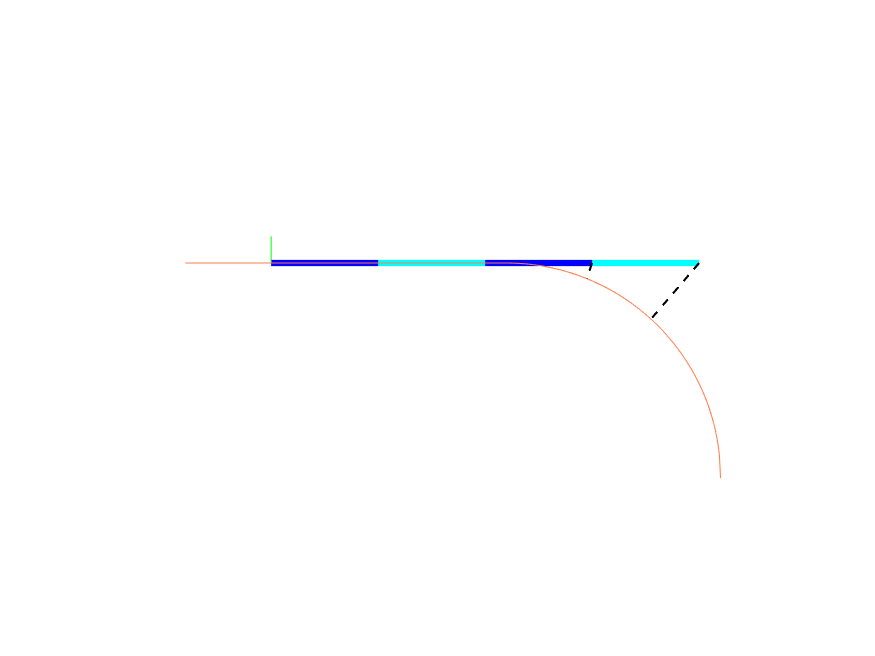
\includegraphics[trim=4cm 3.5cm 2cm 1cm, clip=true, totalheight=0.23\textheight] {figures/case-1-2/goodgirl1.png}}
    \hfil
    \subfloat[$t = 5 s$]{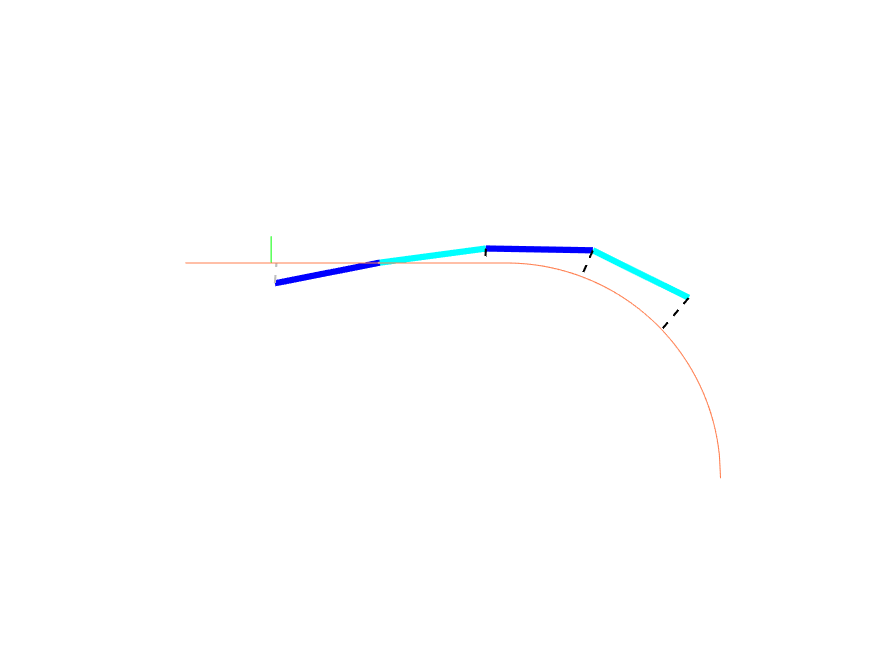
\includegraphics[trim=4cm 3.5cm 2cm 1cm, clip=true, totalheight=0.23\textheight]{figures/case-1-2/goodgirl2.png}}
    
    \subfloat[$t = 10 s$]{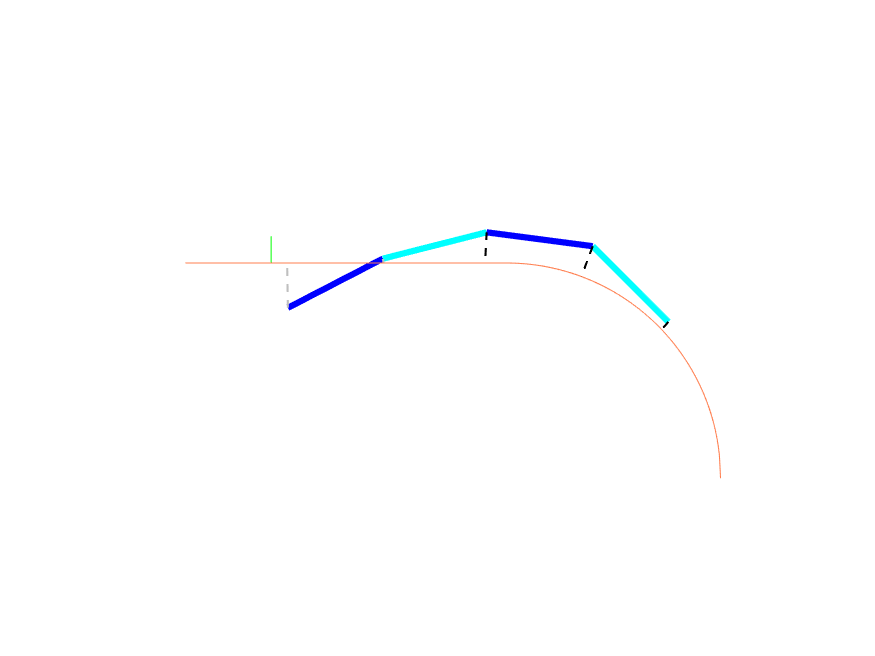
\includegraphics[trim=4cm 3.5cm 2cm 1cm, clip=true, totalheight=0.23\textheight]{figures/case-1-2/goodgirl3.png}}
    
    \caption{Simulation demo - adjusting to path from nearby}
    \label{fig:case1-2a}
\end{figure}

\begin{figure}[H]
    \centering
    
    \subfloat[$t = 0 s$]{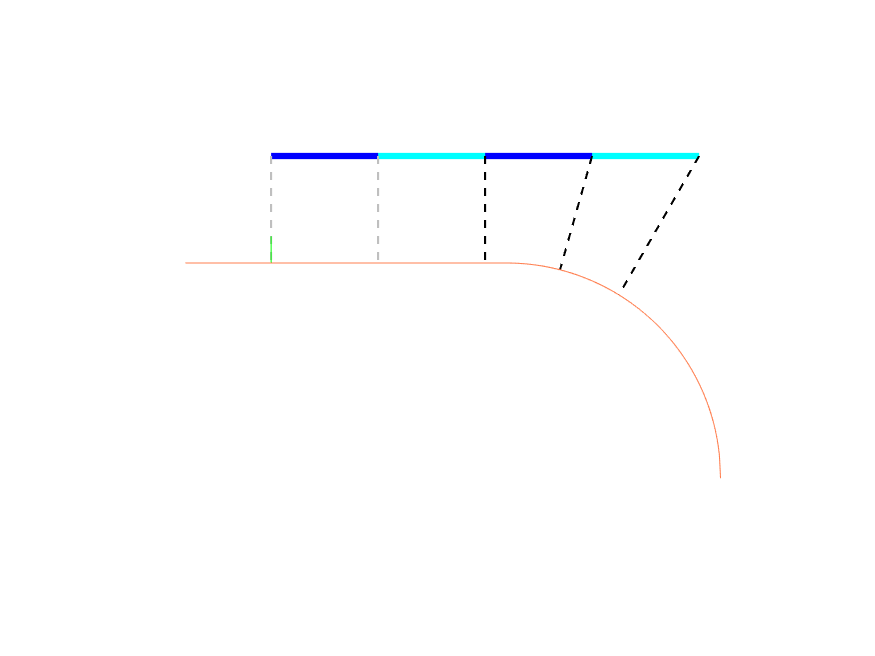
\includegraphics[trim=4cm 3.5cm 2cm 1cm, clip=true, totalheight=0.23\textheight] {figures/case-1-2/badgirl1.png}}
    \hfil
    \subfloat[$t = 5 s$]{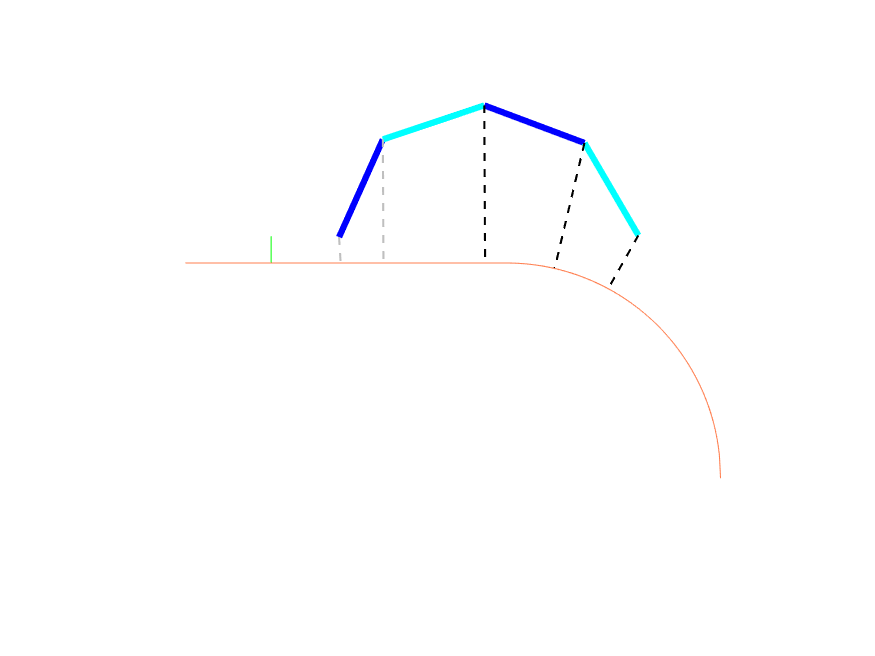
\includegraphics[trim=4cm 3.5cm 2cm 1cm, clip=true, totalheight=0.23\textheight]{figures/case-1-2/badgirl2.png}}
    
    \subfloat[$t = 10 s$]{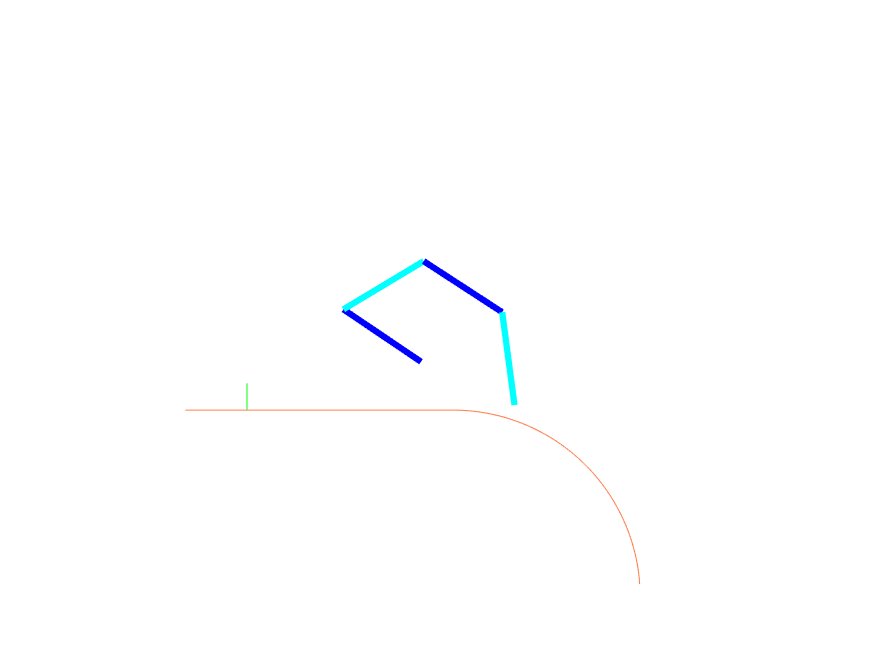
\includegraphics[trim=4cm 3.5cm 2cm 1cm, clip=true, totalheight=0.23\textheight]{figures/case-1-2/badgirl3.png}}
    
    \caption{Simulation demo - adjusting to path from a distance}
    \label{fig:case1-2b}
\end{figure}

It is evident that path adjustment relies on a start configuration close to the path to be successful as well. However, none of the simulations are able to perfectly adjust to the path. An important reason for this is that the robot cannot change the position of its center of mass without friction or push-points (obstacles) in the environment. 

The plots in Figure \ref{fig:case1-2-plot} show the joint angles of the controllable joints during the simulations. The reference angles are plotted with a dashed line.
From the plots it can be observed that the end effector is very close to the path and the corresponding reference angles $q_{d,4}$ are almost met in both cases. Additionally, the reference angles of link 2 and 3 wish to bend the links downward to the path. This is logical, just not completely feasible. A consequence of this is that the robot too far from the path is curling up. 

\begin{figure}[H]
    \centering
    
    \subfloat[Start at $(x_0,y_0) = (0,0)$]{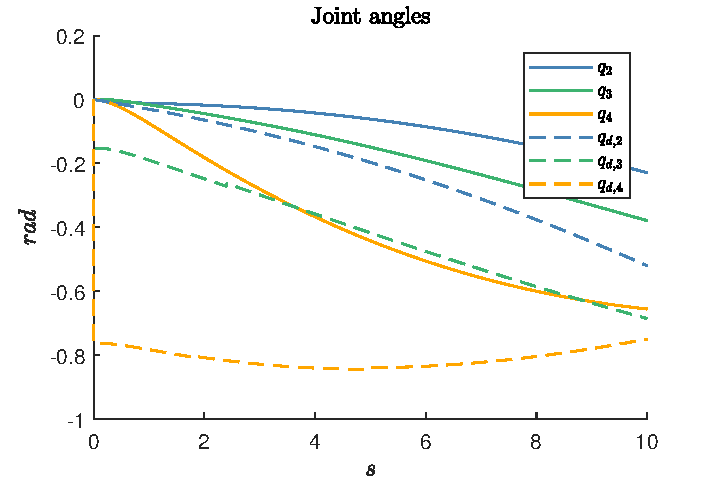
\includegraphics[clip=true, totalheight=0.31\textheight]{figures/case-1-2/case12a.pdf}}

    \subfloat[Start at $(x_0,y_0) = (0,-1)$]{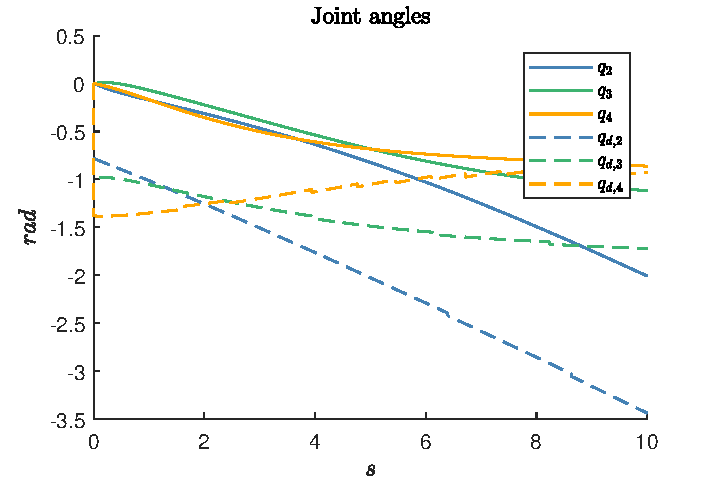
\includegraphics[clip=true, totalheight=0.31\textheight]{figures/case-1-2/case12b.pdf}}

    \caption{Joint angles for path adjustment with different starting configurations}
    \label{fig:case1-2-plot}
\end{figure}


%---------------------------------------------------------------------------------------
%---------------------------------------------------------------------------------------
%---------------------------------------------------------------------------------------

\section{Collision analysis}\label{sec:case3}

This section demonstrates the energy and momentum difference in the robot before and after being influenced by an obstacle. The experiment is performed for validity analysis of the interaction approximations, and the outcome is discussed further in Chapter \ref{ch:discussion}.

\subsection{Single obstacle interaction}\label{subseq:case3}
For simplicity, only one obstacle is included in this experiment. Furthermore, the robot is not set to follow any joint angle references. Instead, a step input torque with magnitude $-0.5Nm$ is applied to the foremost joint for 0.2 seconds. The simulation configuration is given in Table \ref{tab:var-case-3}.

\begin{table}[H]
\centering
    \begin{tabular}{|c|c|c|}
        \hline
         \textbf{Description} & \textbf{Variable name} & \textbf{Value} \\
         \hline \hline
         Simulation time $[s]$& \texttt{simTime} & $3$ \\
         \hline
         Simulation sample time $[s]$& \texttt{h} & $0.001$ \\
         \hline
         Damping ratio & \texttt{zeta} & $2$ \\
         \hline
         Number of links & \texttt{n} & $4$ \\
         \hline
         Initial joint angles $[rad]$ & \texttt{q\char`_0} & $[0, 0, 0, 0]$ \\
         \hline
         Initial position $[m]$ & \texttt{q\char`_0(n+1:n+2)} & $[0, 0]$ \\
         \hline
         Number of obstacles & \texttt{num\char`_obstacles} & $1$ \\         
         \hline
         Obstacle position $[m]$& \texttt{obstacle\char`_coords} & $(3.5, -0.3)$ \\
         \hline
    \end{tabular}
    \caption{Simulation configuration for \ref{subseq:case3}}
    \label{tab:var-case-3}
\end{table}

The torque is chosen to make the foremost robot link collide with the obstacle so that the resulting change in energy and momentum can be observed. The different positions of the robot to different times are illustrated in Figure \ref{fig:case3}. Furthermore, the energy (\ref{eq:kinen}), momentum (\ref{eq:momentum}) and applied torque is plotted in Figure \ref{fig:case3-plot}.


\begin{figure}[H]
    \centering
    
    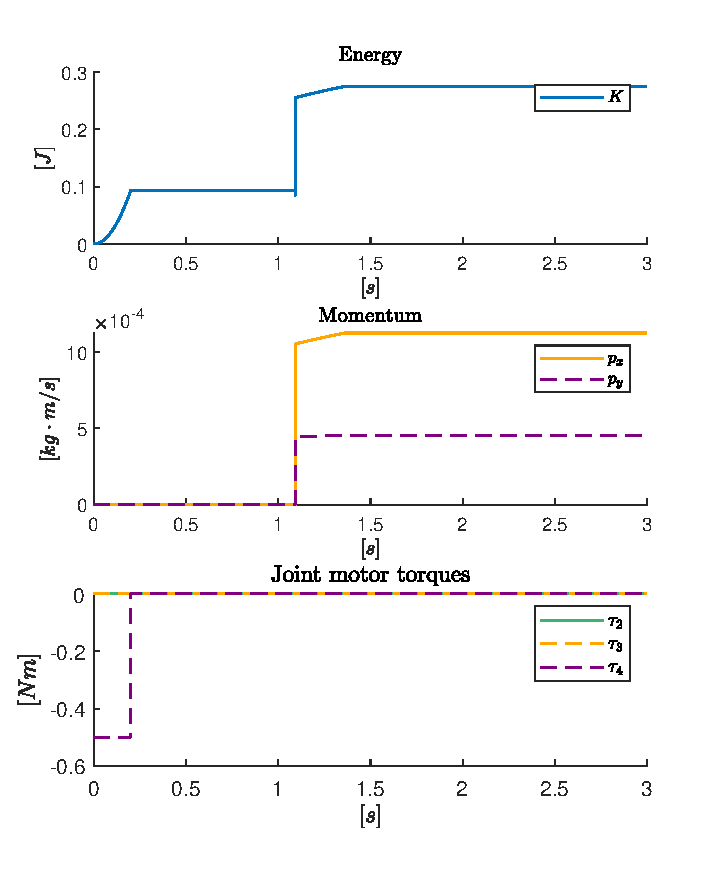
\includegraphics[width=0.85\textwidth]{figures/case-3/energy-momentum.pdf}

    \caption{Energy, momentum and joint motor torques of robot for single collision scenario}
    \label{fig:case3-plot}
\end{figure}


\begin{figure}[H]
    \centering
    
    \subfloat[$t = 0 s$]{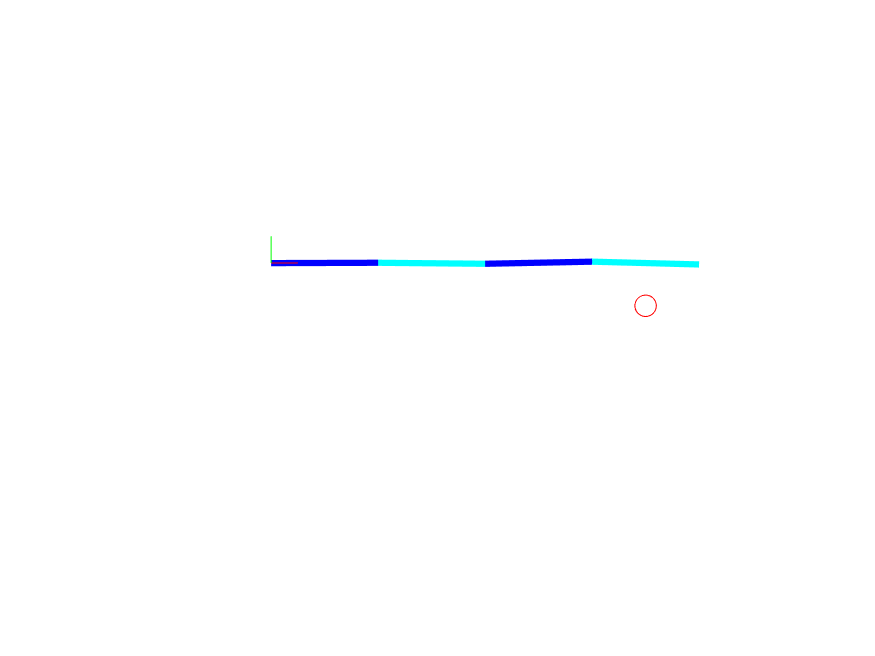
\includegraphics[trim=2cm 4.5cm 2cm 2.8cm, clip=true, width=0.4\textwidth] {figures/case-3/sim1.png}}
    \hfil
    \subfloat[$t = 1 s$]{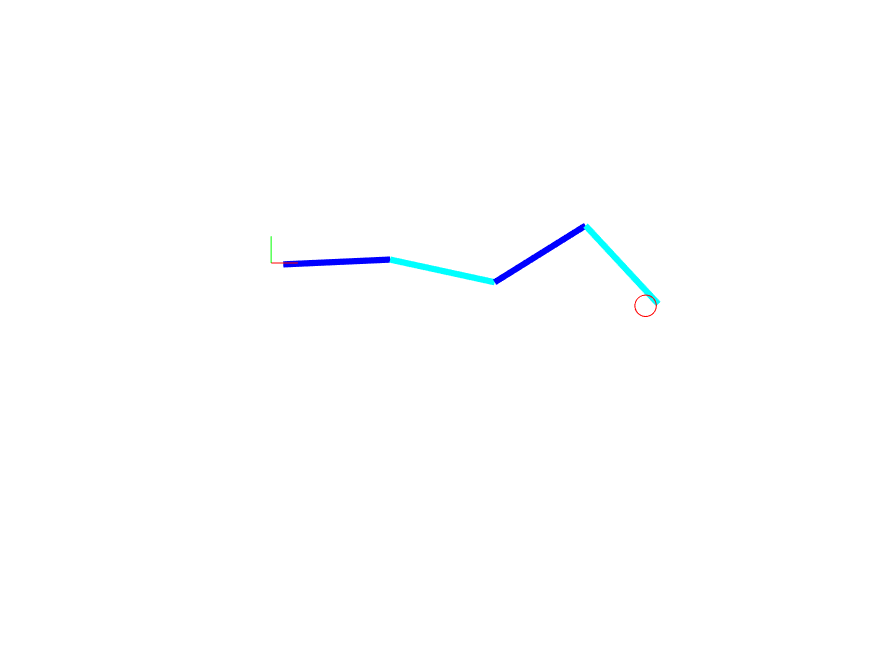
\includegraphics[trim=2cm 4.5cm 2cm 2.8cm, clip=true, width=0.4\textwidth]{figures/case-3/sim2.png}}
    
    \subfloat[$t = 2 s$]{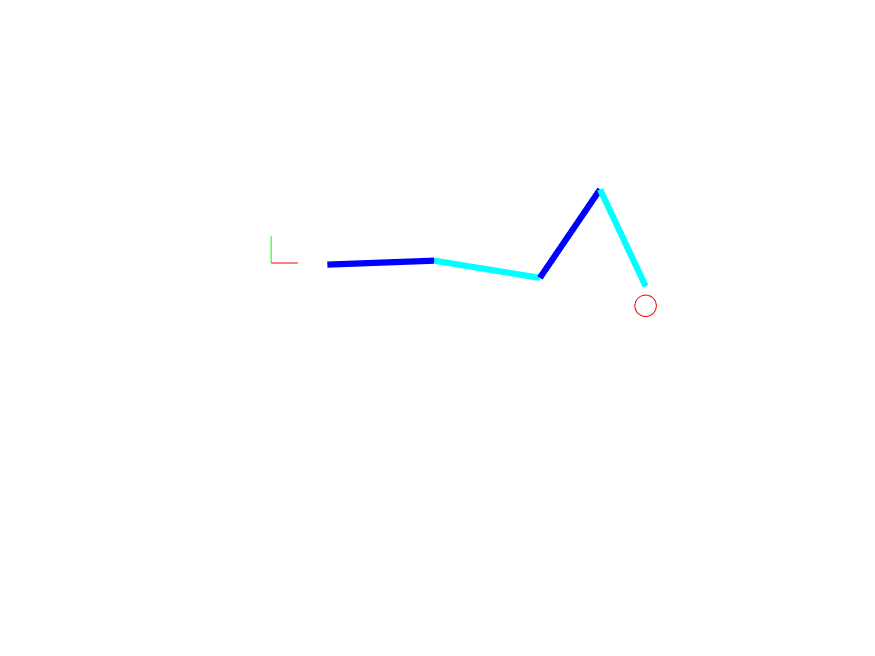
\includegraphics[trim=2cm 4.5cm 2cm 2.8cm, clip=true, width=0.4\textwidth]{figures/case-3/sim3.png}}
    \hfil
    \subfloat[$t = 3 s$]{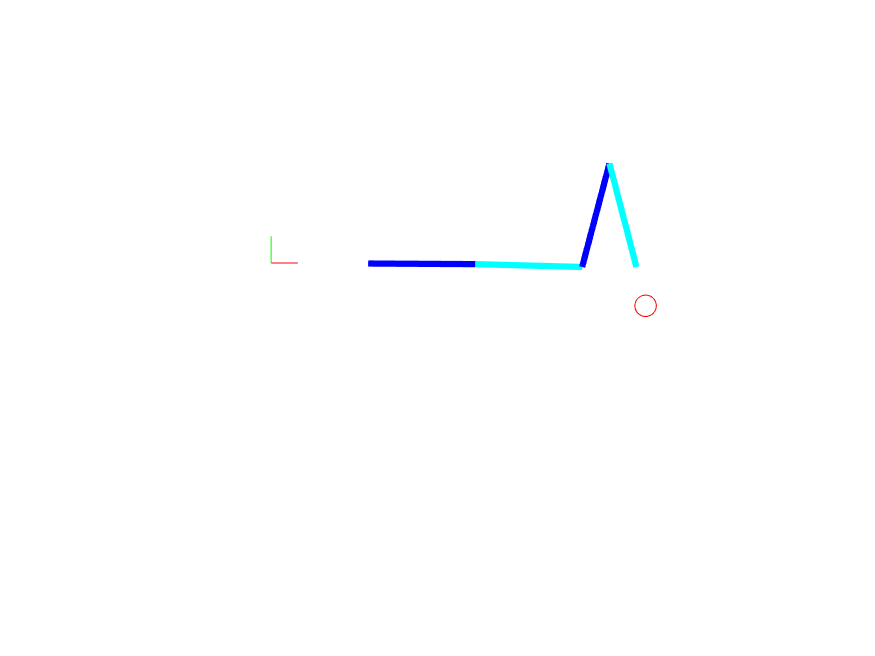
\includegraphics[trim=2cm 4.5cm 2cm 2.8cm, clip=true, width=0.4\textwidth]{figures/case-3/sim4.png}}

    \caption{Simulation demo - interaction with single obstacle}
    \label{fig:case3}
\end{figure}





The motor torque will naturally increase the energy of the robot for the time period in which it is applied. According to laws of physics, the energy level should then stay constant as long as no work is done on the robot and it is moving in a frictionless environment. The energy plot in Figure \ref{fig:case3-plot} confirms this, seeing as the energy stays constant between 0.2 to 1.1 seconds. When the robot then hits the obstacle, a clear change in energy is observed. The approximate time of this collision is further confirmed by the configuration of the robot at 1 seconds seen in part (b) of Figure \ref{fig:case3}.
In reality, the robot would at this point loose energy to the obstacle. From the plot it can however be observed that the energy is increased until the robot link no longer is in contact with the obstacle.
The total energy of the robot before the contact is $0.0933J$ and $0.2751J$ after the contact, meaning the energy is increased by 295\%.

Furthermore, 
%the total momentum of a closed system of bodies should be conserved. Seeing as the obstacle neither has any mass nor velocity, the only body with momentum in this system is the snake robot. Hence, 
the momentum of the snake robot should be conserved despite the collision (see \ref{subseq:momentum}). However, it turns out that the momentum in x-direction increases by $1.1271kg\cdot m/s$ and the momentum in y-direction increases by $0.4519kg\cdot m/s$, violating the well known \textit{law of conservation of momentum}.

It should be noted that the robot cannot change the position of its center of mass without an external force. Therefore, even though the links obtain velocities after the torque is applied, they cancel each other out in the respective directions. The moments in the two directions are determined by the velocities and accordingly unchanged by the torque, as seen in the momentum plot in Figure \ref{fig:case3-plot}.


%---------------------------------------------------------------------------------------
%---------------------------------------------------------------------------------------
%---------------------------------------------------------------------------------------

\section{OAL simulation scenarios}

\subsection{Simple propulsion}\label{subseq:case21}

This scenario aims at demonstrating the concept of OAL. The snake robot is simply set to bend its front joint to $-\pi/2$ while the other joints are to remain in a stretched out configuration. The simulator variable configuration can be seen in Table \ref{tab:var-case-2-1}.

The setpoints are manually determined based on the knowledge that the bending link will collide with an obstacle in trying to obtain the desired angle. Hence, the link will apply a force to the obstacle underneath and consequently drag the whole robot body in the positive $x$ (rightward) direction. A sequence of the movement is presented in Figure \ref{fig:case2-1}. 

\begin{table}[H]
\centering
    \begin{tabular}{|c|c|c|}
        \hline
         \textbf{Description} & \textbf{Variable name} & \textbf{Value} \\
         \hline \hline
         Simulation time $[s]$& \texttt{simTime} & $20$ \\
         \hline
         Simulation sample time $[s]$& \texttt{h} & $0.001$ \\
         \hline
         Damping ratio & \texttt{zeta} & $2$ \\
         \hline
         Number of links & \texttt{n} & $4$ \\
         \hline
         Joint angle setpoints $[rad]$ & \texttt{q\char`_ref} & $[0, 0, 0, -\pi/2]$ \\
         \hline
         Initial joint angles $[rad]$ & \texttt{q\char`_0} & $[0, 0, 0, 0]$ \\
         \hline
         Initial position $[m]$ & \texttt{q\char`_0(n+1:n+2)} & $[0, 0]$ \\
         \hline
         Number of obstacles & \texttt{num\char`_obstacles} & $3$ \\         
         \hline
         Obstacle positions $[m]$& \texttt{obstacle\char`_coords} & \makecell{$(0.8, -0.08)$ \\ $(1.6, 0.08)$ \\ $(3.3, -0.3)$} \\
         \hline
    \end{tabular}
    \caption{Simulation configuration for \ref{subseq:case21}}
    \label{tab:var-case-2-1}
\end{table}

The obstacles laying close to the rear links are positioned to allow the rest of the robot to stay flat. From Figure \ref{fig:case2-1} it can be seen that the robot moves away from the obstacles towards the end without pushing against anything. This is a consequence of the modeled frictionless environment.

From the plots in Figure \ref{fig:case2-1-plot} it is clear that the collision with the lower obstacle takes place at approximately 3 seconds. At this point, the joint velocities are projected such that the front link does not cross the obstacle. Additionally, the preceding joints experience an offset as the front joint applies a torque that influences the whole robot.

A repercussion of the geometrical approximation of the contact forces becomes obvious in this experiment. The joint velocities in the emphasised time span in part (b) of Figure \ref{fig:case2-1-plot} admit a twitching behaviour as a result of the velocity projections. This circumstance is discussed in Chapter \ref{ch:discussion}.

\begin{figure}[H]
    \centering
    
    \subfloat[$t = 0 s$]{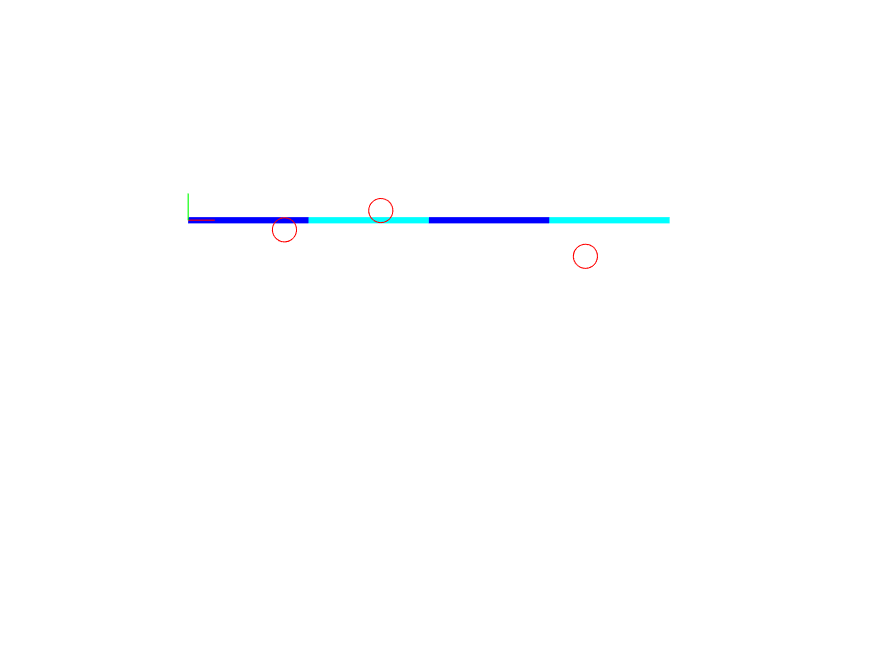
\includegraphics[trim=2cm 4cm 2cm 1.5cm, clip=true, totalheight=0.18\textheight] {figures/case-2-1/sim1.png}}
    \hfil
    \subfloat[$t = 4 s$]{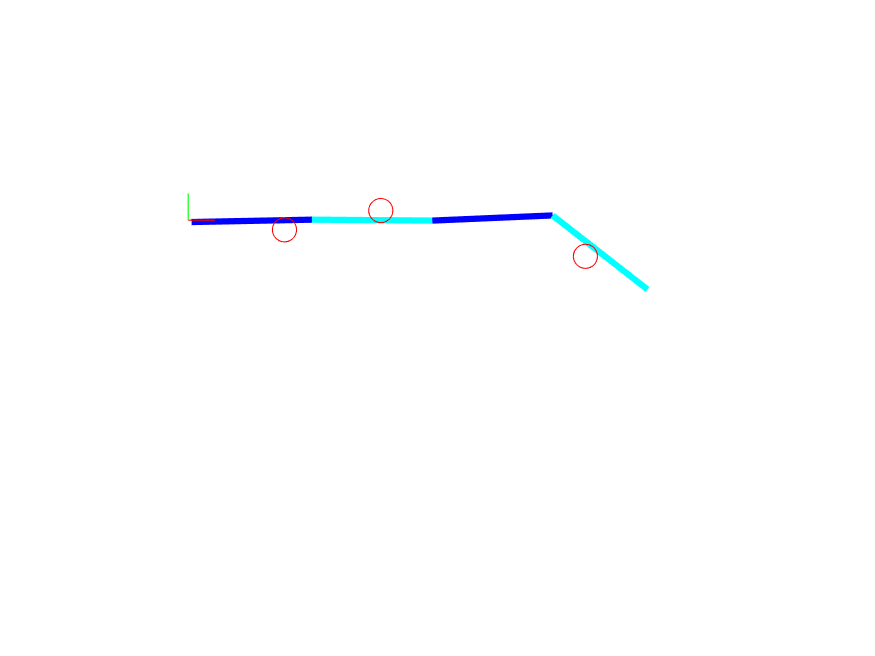
\includegraphics[trim=2cm 4cm 2cm 1.5cm, clip=true, totalheight=0.18\textheight]{figures/case-2-1/sim2.png}}
    
    \subfloat[$t = 8 s$]{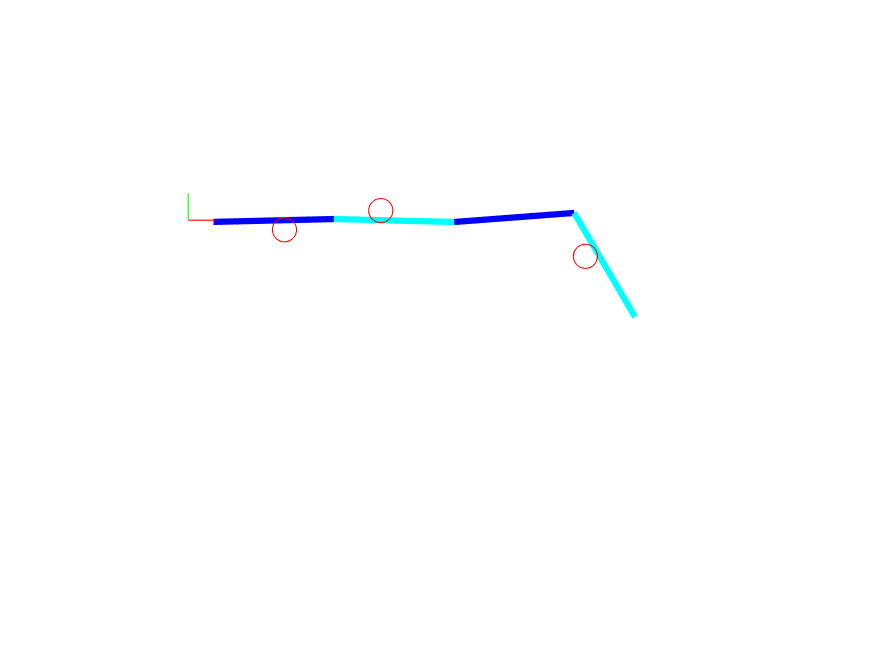
\includegraphics[trim=2cm 4cm 2cm 1.5cm, clip=true, totalheight=0.18\textheight]{figures/case-2-1/sim3.png}}
    \hfil
    \subfloat[$t = 12 s$]{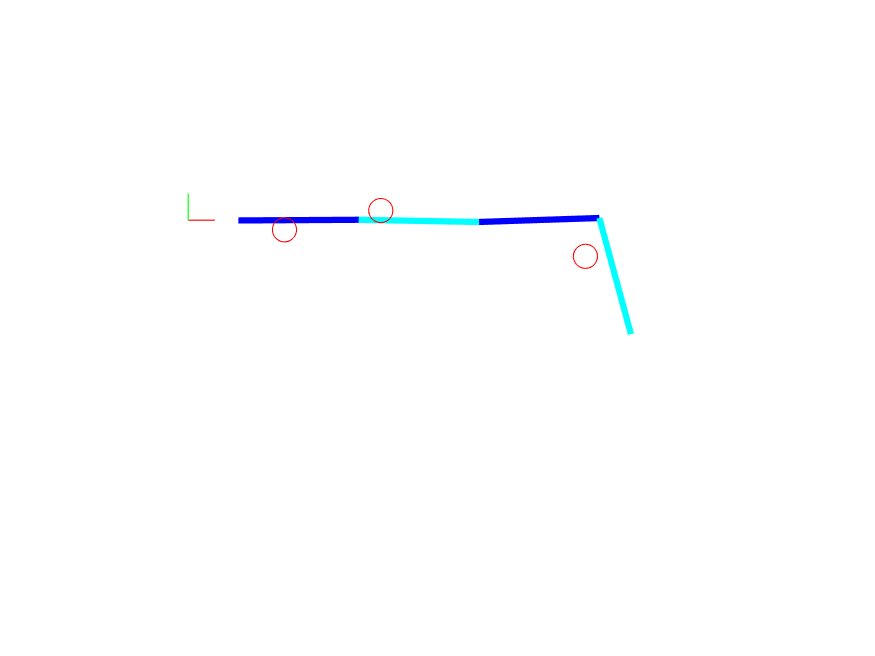
\includegraphics[trim=2cm 4cm 2cm 1.5cm, clip=true, totalheight=0.18\textheight]{figures/case-2-1/sim4.png}}

    \subfloat[$t = 16 s$]{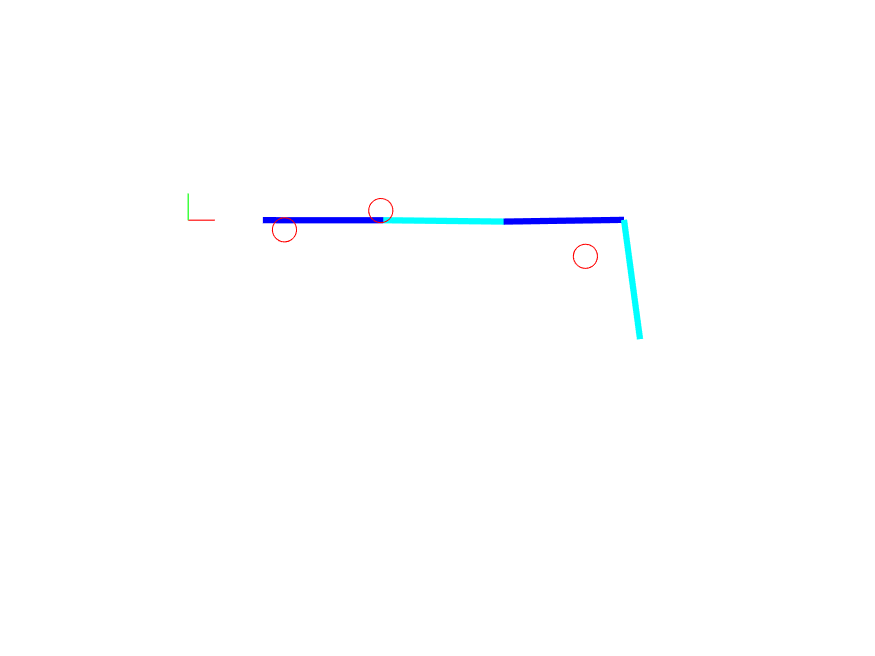
\includegraphics[trim=2cm 4cm 2cm 1.5cm, clip=true, totalheight=0.18\textheight]{figures/case-2-1/sim5.png}}
    \hfil
    \subfloat[$t = 20 s$]{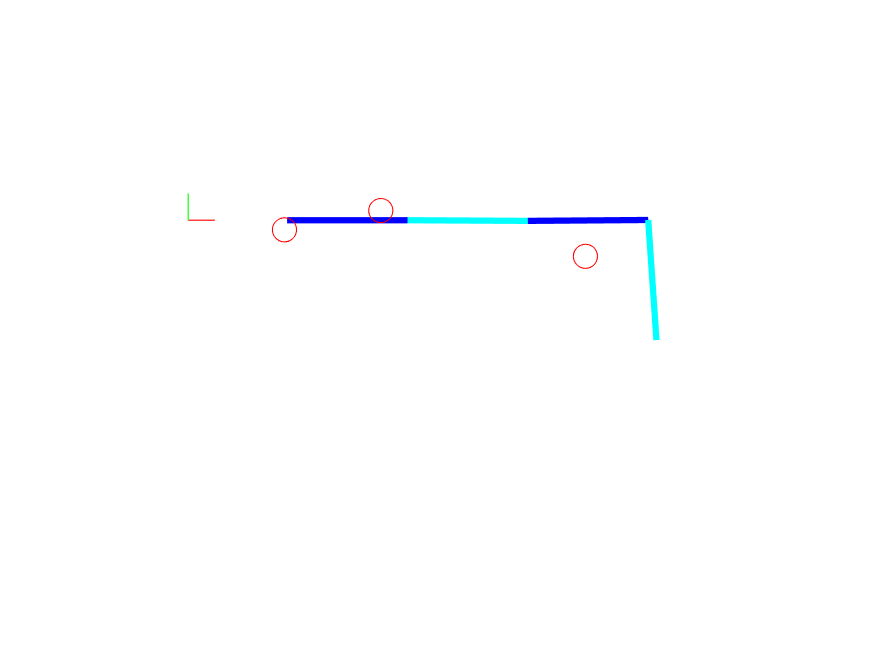
\includegraphics[trim=2cm 4cm 2cm 1.5cm, clip=true, totalheight=0.18\textheight]{figures/case-2-1/sim6.png}}

    \caption{Simulation demo - propulsion with static joint setpoint}
    \label{fig:case2-1}
\end{figure}





\begin{figure}[H]
    \centering
    
    \subfloat[]{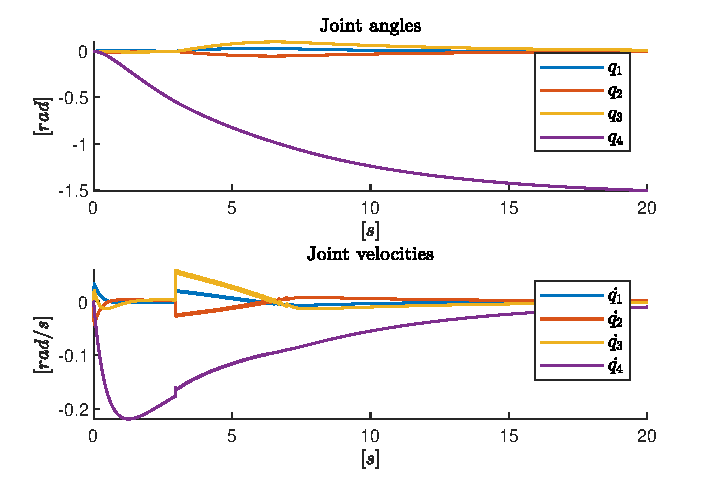
\includegraphics[clip=true, totalheight=0.4\textheight]{figures/case-2-1/case21.pdf}}

    \subfloat[Zoom of joint velocities in seconds 5-10]{\fbox{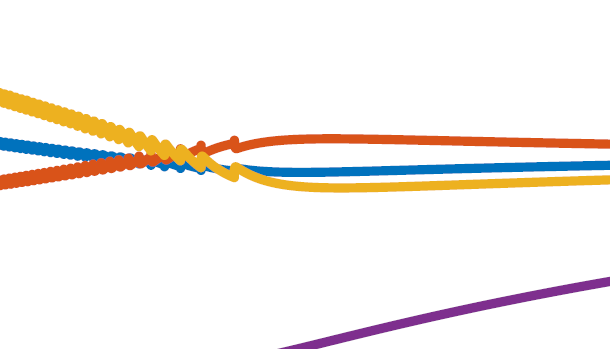
\includegraphics[clip=true, totalheight=0.12\textheight]{figures/case-2-1/zoom21.PNG}}}

    \caption{Joint angles and velocities for the single setpoint scenario}
    \label{fig:case2-1-plot}
\end{figure}


%---------------------------------------------------------------------------------------
%---------------------------------------------------------------------------------------
\clearpage
\subsection{Obstacle interaction without propulsion}\label{subseq:case22}

Seeing as propulsion requires a force in the respective direction, there are scenarios where a set of joint torques are insufficient for attaining this force. This scenario aims at illustrating the case where the forces applied work against each other in the direction of propulsion and the robot is simply deformed. The variable configuration for the simulation is presented in Table \ref{tab:var-case-2-2} and Figure \ref{fig:case2-2} shows a sequence of the motion.


\begin{table}[H]
\centering
    \begin{tabular}{|c|c|c|}
        \hline
         \textbf{Description} & \textbf{Variable name} & \textbf{Value} \\
         \hline \hline
         Simulation time $[s]$& \texttt{simTime} & $9$ \\
         \hline
         Simulation sample time $[s]$ & \texttt{h} & $0.001$ \\
         \hline
         Damping ratio & \texttt{zeta} & $1$ \\
         \hline
         Number of links & \texttt{n} & $3$ \\
         \hline
         Joint angle setpoints $[rad]$& \texttt{q\char`_ref} & $[0, -\pi/3, \pi/3]$ \\
         \hline
         Initial joint angles $[rad]$& \texttt{q\char`_0} & $[0, 0, 0]$ \\
         \hline
         Initial position $[m]$ & \texttt{q\char`_0(n+1:n+2)} & $[0, 0]$ \\
         \hline
         Number of obstacles & \texttt{num\char`_obstacles} & $3$ \\         
         \hline
         Obstacle positions $[m]$& \texttt{obstacle\char`_coords} & \makecell{$(0.5, 0.1)$ \\ $(1.5, -0.1)$ \\ $(2.5, 0.1)$} \\
         \hline
    \end{tabular}
    \caption{Simulation configuration for \ref{subseq:case22}}
    \label{tab:var-case-2-2}
\end{table}


\begin{figure}[H]
    \centering
    
    \subfloat[$t = 0 s$]{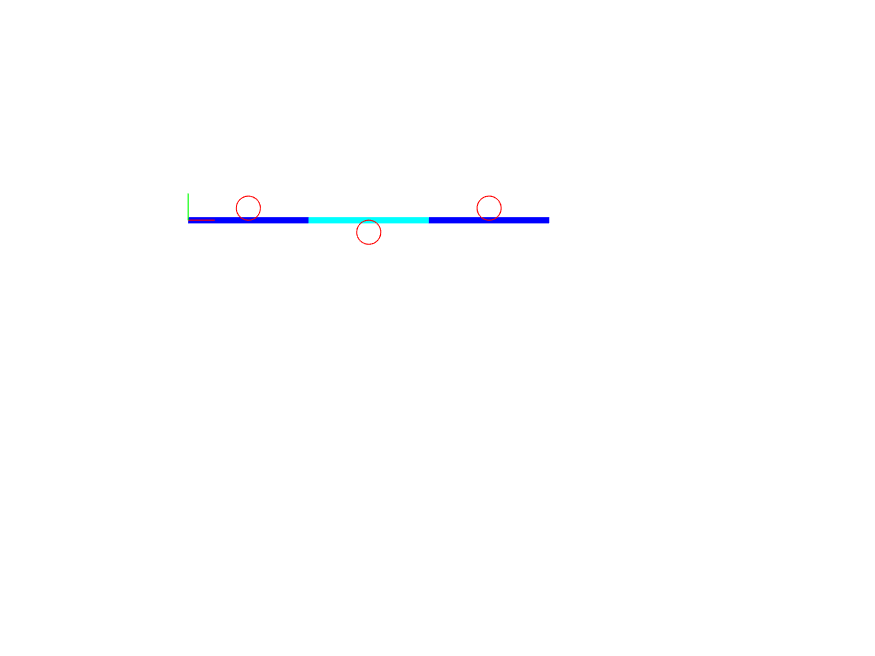
\includegraphics[trim=2cm 4cm 2cm 1.5cm, clip=true, totalheight=0.16\textheight] {figures/case-2-2/2sim1.png}}
    \hfil
    \subfloat[$t = 3 s$]{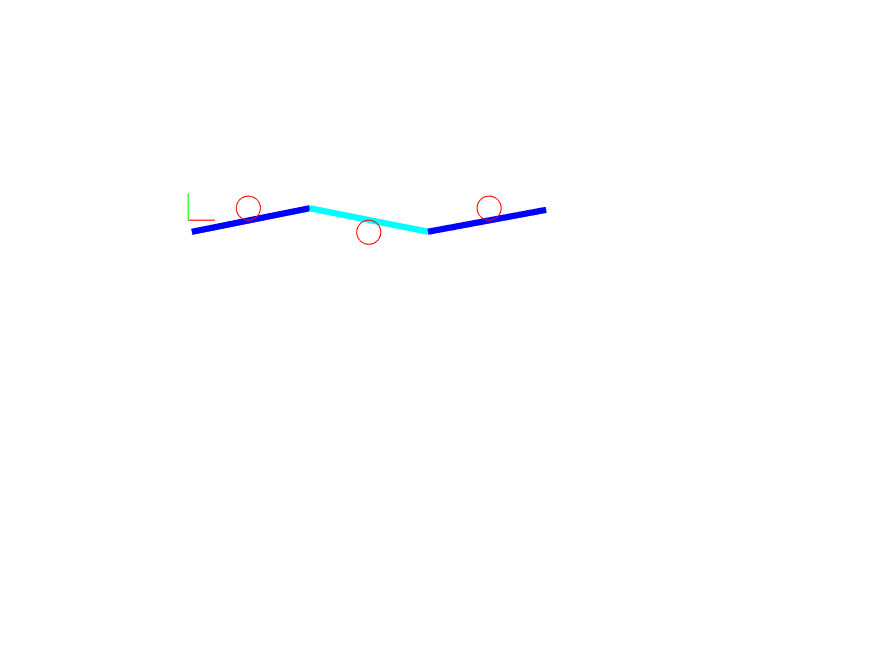
\includegraphics[trim=2cm 4cm 2cm 1.5cm, clip=true, totalheight=0.16\textheight]{figures/case-2-2/2sim2.png}}
    
    \subfloat[$t = 6 s$]{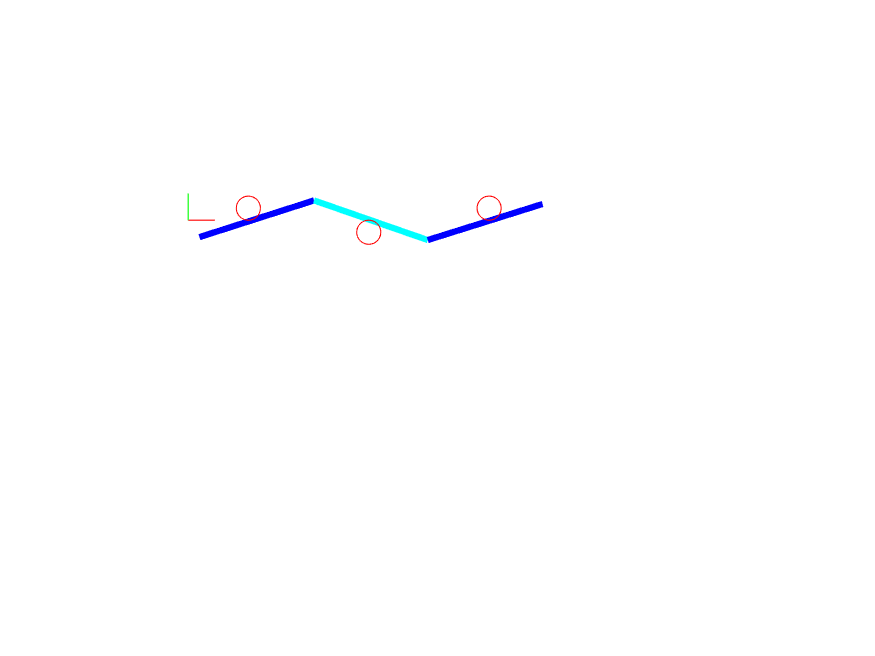
\includegraphics[trim=2cm 4cm 2cm 1.5cm, clip=true, totalheight=0.16\textheight]{figures/case-2-2/2sim3.png}}
    \hfil
    \subfloat[$t = 9 s$]{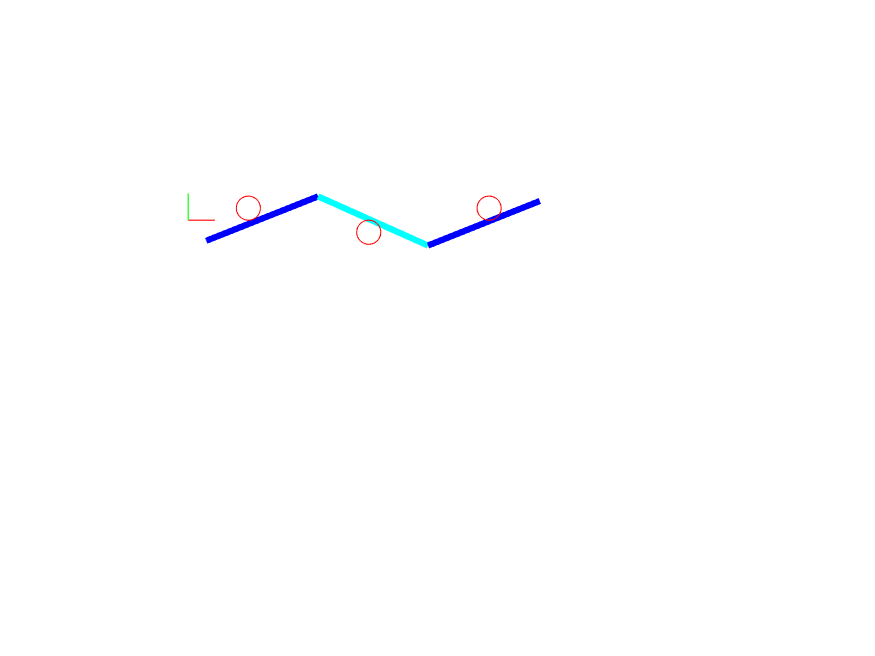
\includegraphics[trim=2cm 4cm 2cm 1.5cm, clip=true, totalheight=0.16\textheight]{figures/case-2-2/2sim4.png}}
    
    \caption{Simulation demo - no propulsion}
    \label{fig:case2-2}
\end{figure}



%---------------------------------------------------------------------------------------
%---------------------------------------------------------------------------------------

\subsection{Unsuccessful propulsion attempt along path}\label{subseq:case24}

This experiment demonstrates a case in which the simplifications made are preventing the robot from moving in the desired direction. The robot is at all times merely set to adjust itself to the path without any objective of propulsion. Just like in \ref{subseq:case21}, the obstacles blocking the robot are the factor leading to propulsion. The configuration is summarized in Table \ref{tab:var-case-2-4}, and the desired path (\ref{eq:path}) is the same one as in \ref{subseq:case12}.

\begin{table}[H]
\centering
    \begin{tabular}{|c|c|c|}
        \hline
         \textbf{Description} & \textbf{Variable name} & \textbf{Value} \\
         \hline \hline
         Simulation time $[s]$ & \texttt{simTime} & $60$ \\
         \hline
         Simulation sample time $[s]$ & \texttt{h} & $0.005$ \\
         \hline
         Damping ratio & \texttt{zeta} & $2$ \\
         \hline
         Number of links & \texttt{n} & $5$ \\
         \hline
         Joint angle setpoints $[rad]$& \texttt{q\char`_ref} & \makecell{Given by the path \\projection method}  \\
         \hline
         Initial joint angles $[rad]$ & \texttt{q\char`_0} & $[0, 0, 0, 0, 0]$ \\
         \hline
         Initial position $[m]$ & \texttt{q\char`_0(n+1:n+2)} & $[-1, 0]$ \\
         \hline
         Number of obstacles & \texttt{num\char`_obstacles} & $3$ \\         
         \hline
         Obstacle positions $[m]$& \texttt{obstacle\char`_coords} & \makecell{$(0.6, -0.1)$ \\ $(1.6, 0.1)$ \\ $(3.2, -0.33)$} \\
         \hline
    \end{tabular}
    \caption{Simulation configuration for \ref{subseq:case24}}
    \label{tab:var-case-2-4}
\end{table}

The resulting problem is caused by the path projection method that disregards the positioning of the tail. When the tail bends over an obstacle, the resulting contact force pushes the robot in the wrong direction while the front link is pushing it in the right direction. The result is that the robot gets stuck. A sequence of the movement is presented in Figure \ref{fig:case2-4}.

\begin{figure}[H]
    \centering
    
    \subfloat[$t = 0 s$]{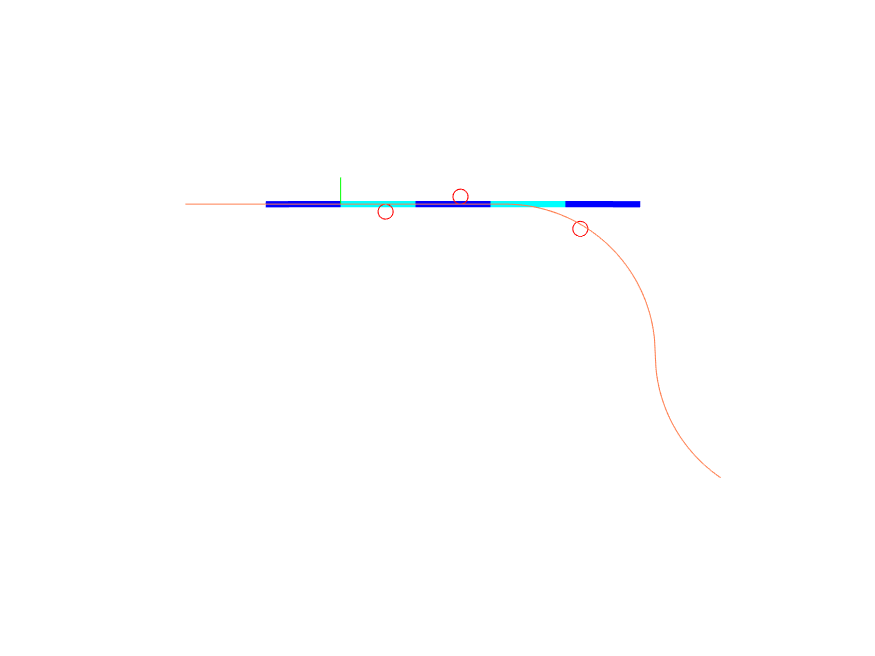
\includegraphics[trim=2.5cm 3cm 2cm 3cm, clip=true, width=0.4\textwidth] {figures/case-2-4/sim1.png}}
    \hfil
    \subfloat[$t = 20 s$]{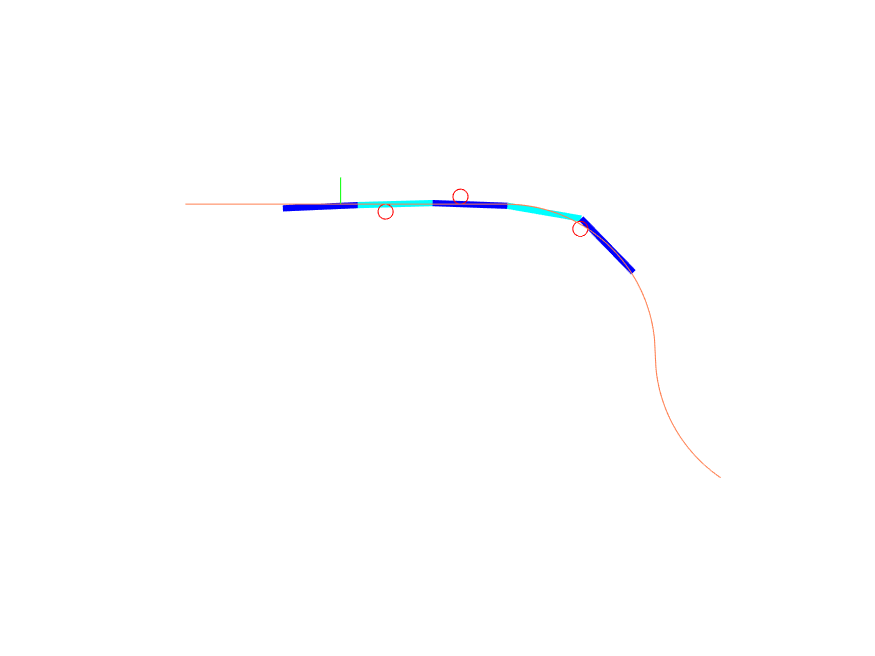
\includegraphics[trim=2.5cm 3cm 2cm 3cm, clip=true, width=0.4\textwidth]{figures/case-2-4/sim2.png}}
    
    \subfloat[$t = 40 s$]{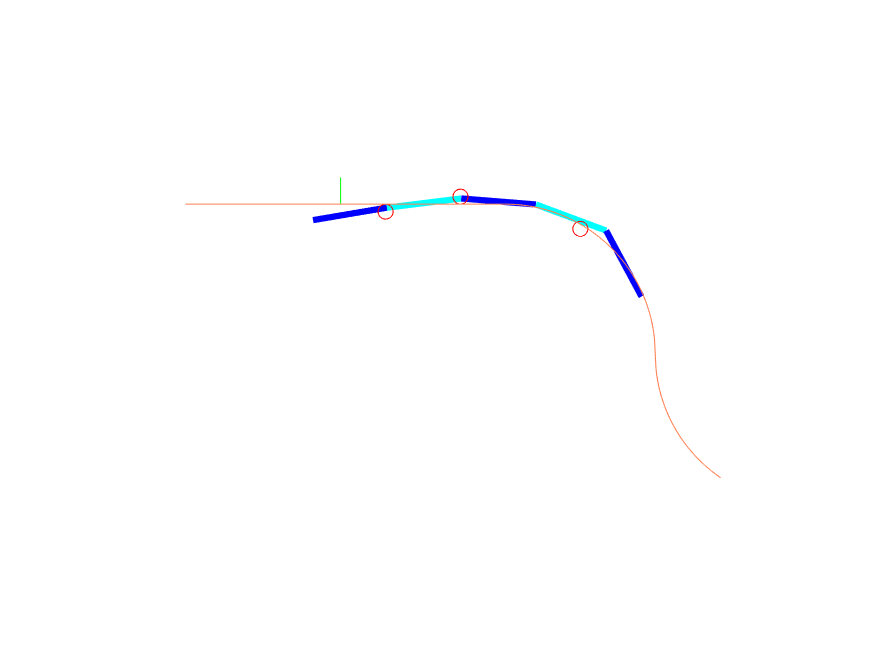
\includegraphics[trim=2.5cm 3cm 2cm 3cm, clip=true, width=0.4\textwidth]{figures/case-2-4/sim3.png}}
    \hfil
    \subfloat[$t = 60 s$]{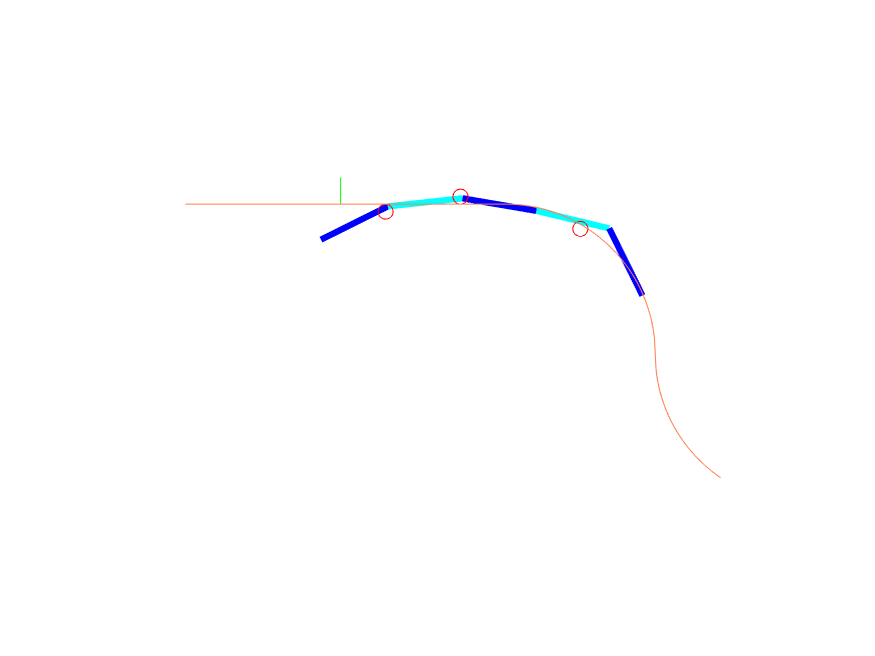
\includegraphics[trim=2.5cm 3cm 2cm 3cm, clip=true, width=0.4\textwidth]{figures/case-2-4/sim4.png}}

    \caption{Simulation demo - failed propulsion along path}
    \label{fig:case2-4}
\end{figure}







%---------------------------------------------------------------------------------------
%---------------------------------------------------------------------------------------


\subsection{Propulsion along path}\label{subseq:case23}

This case is to illustrate how the robot can aid obstacles to propel along a predefined path. Since the robot is only position controlled based on deviation from the path, the obstacles are placed in a manner that supports both the desired shape and motion. The two obstacles in the middle are to keep the rear links on the path, while the obstacle in front is placed so that the robot can push against it and pull itself forward. In order for this to happen, the obstacle has been placed slightly on the path like in previous experiments, leading to a constant deviation from the path. The robot's desire to always stay as close to the path as possible makes it push against the obstacle.

The leftmost obstacle is added based on the observations made in \ref{subseq:case24}, where the tail deviated from the path and caused the robot to get stuck. The tail link will now be pushed back to the path when in contact with this obstacle. An important point to note is that the spacing between the two leftmost obstacles violates assumption 10 in \ref{seq:assumptions}, saying that every link is in contact with at most one obstacle. The simulator is however able to handle this scenario and compute contact Jacobians and projection matrices (see \ref{subseq:HPFC}-\ref{subseq:mult_contacts}) for both contact points.

The variable configurations are presented in Table \ref{tab:var-case-2-3} and the desired path (\ref{eq:path}) is the same one as in \ref{subseq:case12}.


\begin{table}[H]
\centering
    \begin{tabular}{|c|c|c|}
        \hline
         \textbf{Description} & \textbf{Variable name} & \textbf{Value} \\
         \hline \hline
         Simulation time $[s]$ & \texttt{simTime} & $120$ \\
         \hline
         Simulation sample time $[s]$ & \texttt{h} & $0.005$ \\
         \hline
         Damping ratio & \texttt{zeta} & $1$ \\
         \hline
         Number of links & \texttt{n} & $5$ \\
         \hline
         Joint angle setpoints $[rad]$& \texttt{q\char`_ref} & \makecell{Given by the path \\projection method}  \\
         \hline
         Initial joint angles $[rad]$ & \texttt{q\char`_0} & $[0, 0, 0, 0, 0]$ \\
         \hline
         Initial position $[m]$ & \texttt{q\char`_0(n+1:n+2)} & $[-1, 0]$ \\
         \hline
         Number of obstacles & \texttt{num\char`_obstacles} & $4$ \\         
         \hline
         Obstacle positions $[m]$& \texttt{obstacle\char`_coords} & \makecell{$(-0.1, -0.1)$ \\ $(0.6, -0.1)$ \\ $(1.6, 0.1)$ \\ $(3.2, -0.33)$} \\
         \hline
    \end{tabular}
    \caption{Simulation configuration for \ref{subseq:case23}}
    \label{tab:var-case-2-3}
\end{table}

The movement is shown in Figure \ref{fig:case2-3}, where it can be seen that the robot follows the path as long as it has sufficiently many obstacles to push against. At 40 seconds the robot starts moving slightly through the radius of the third obstacle. This is an effect of the projection of the joint velocities.

\begin{figure}
    \centering
    
    \subfloat[$t = 0 s$]{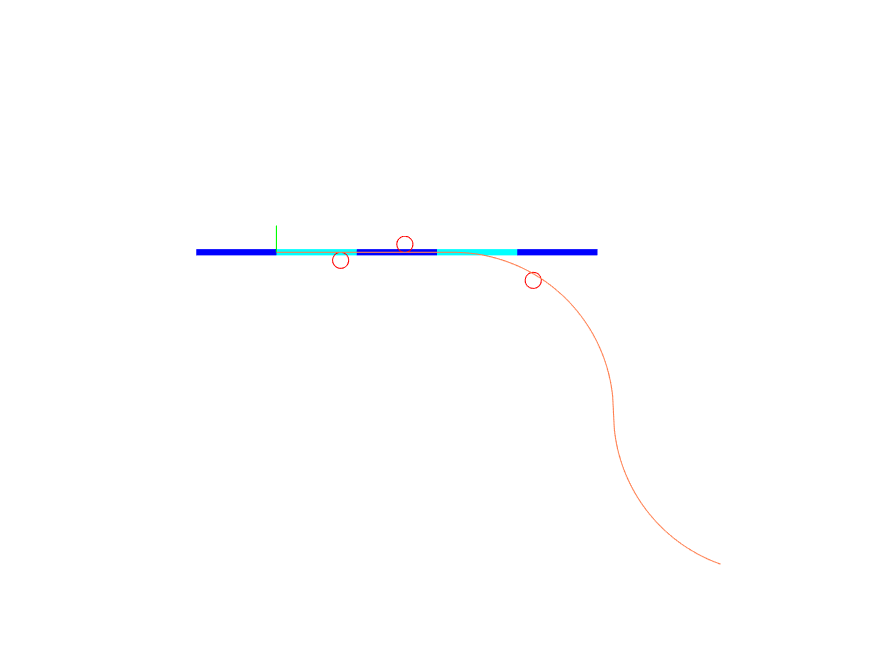
\includegraphics[trim=2cm 3cm 2cm 3cm, clip=true, totalheight=0.15\textheight] {figures/case-2-3/sim1.png}}
    \hfil
    \subfloat[$t = 20 s$]{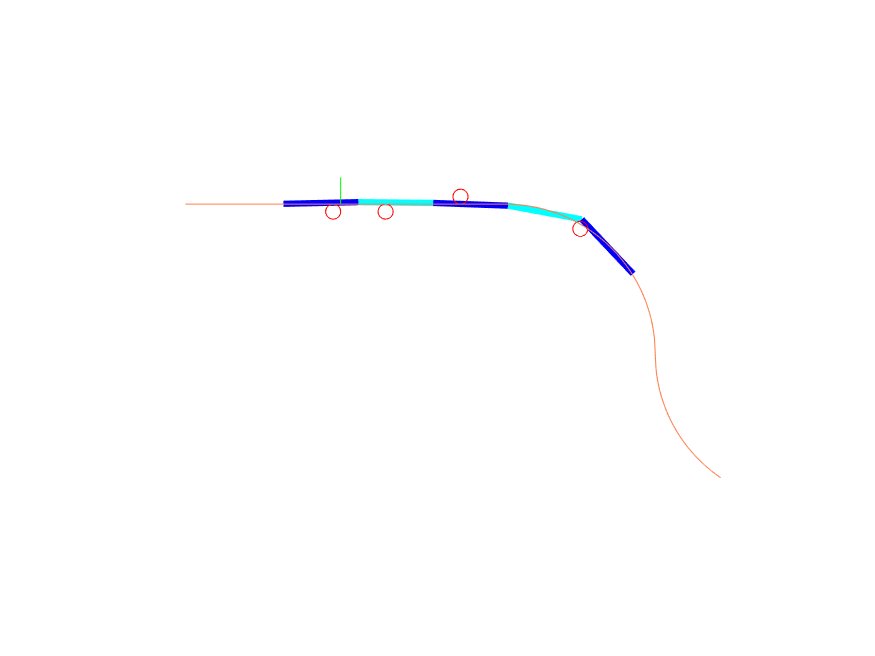
\includegraphics[trim=2cm 3cm 2cm 3cm, clip=true, totalheight=0.15\textheight]{figures/case-2-3/sim2.png}}
    
    \subfloat[$t = 40 s$]{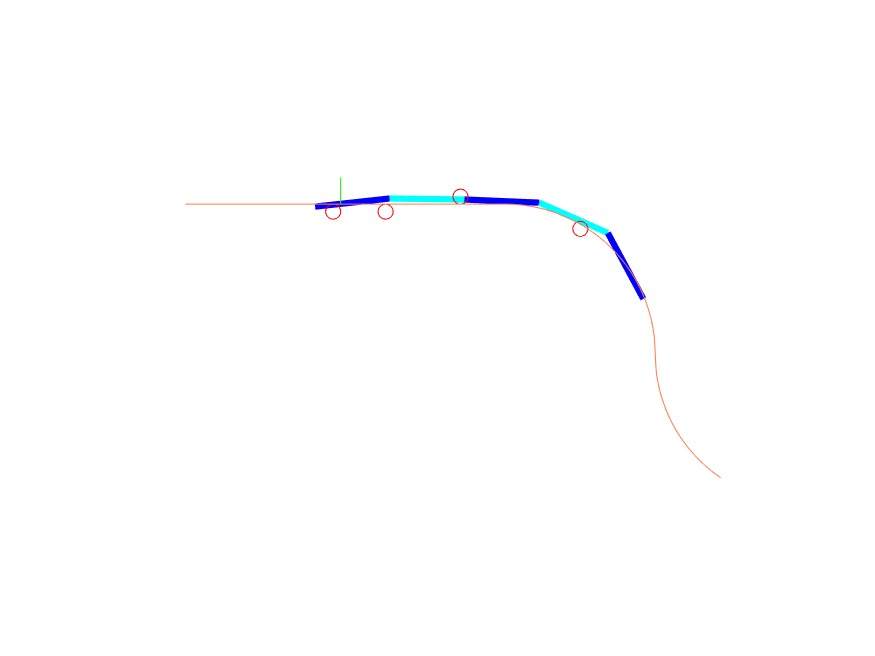
\includegraphics[trim=2cm 3cm 2cm 3cm, clip=true, totalheight=0.15\textheight]{figures/case-2-3/sim3.png}}
    \hfil
    \subfloat[$t = 60 s$]{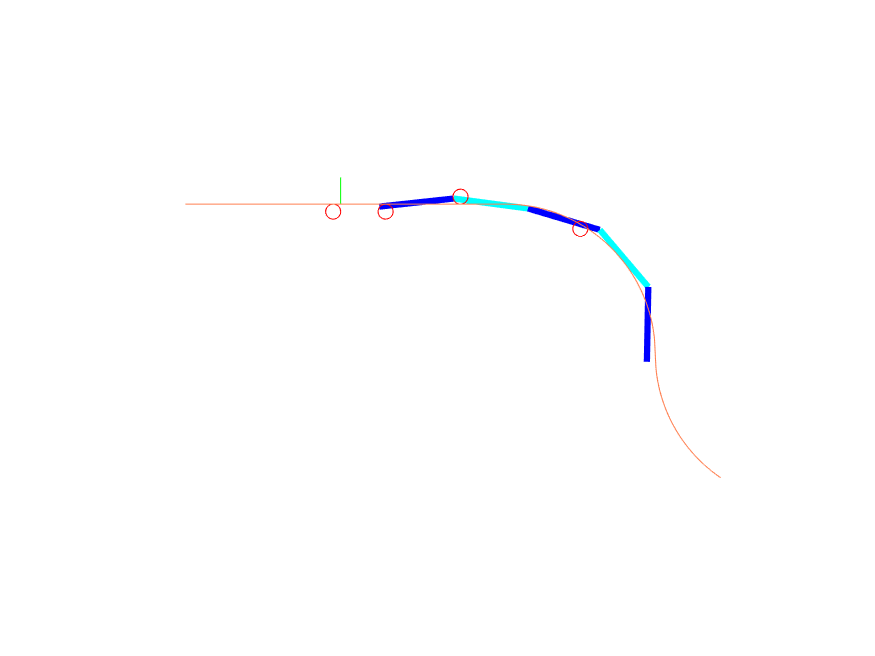
\includegraphics[trim=2cm 3cm 2cm 3cm, clip=true, totalheight=0.15\textheight]{figures/case-2-3/sim4.png}}

    \subfloat[$t = 80 s$]{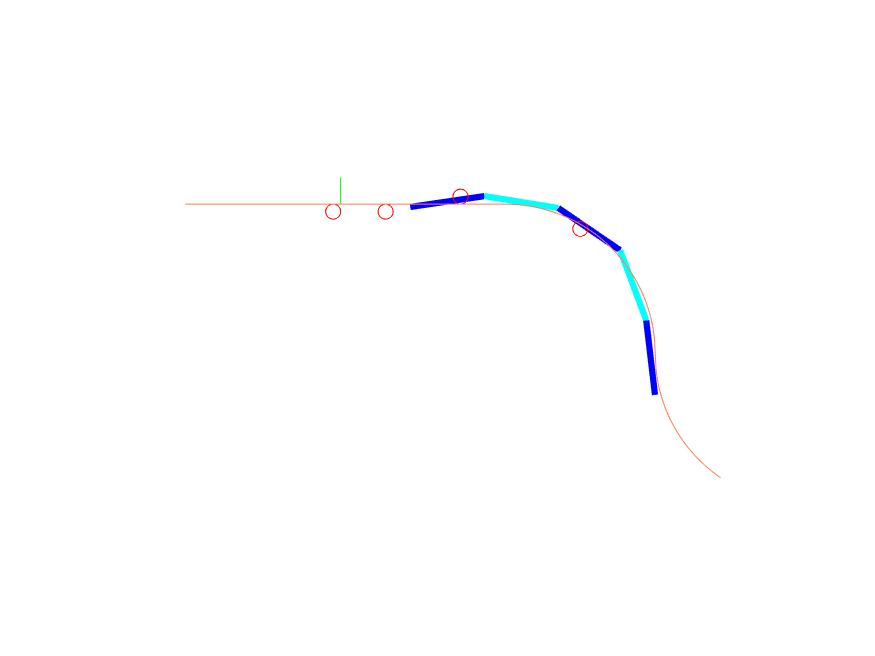
\includegraphics[trim=2cm 3cm 2cm 3cm, clip=true, totalheight=0.15\textheight]{figures/case-2-3/sim5.png}}
    \hfil
    \subfloat[$t = 100 s$]{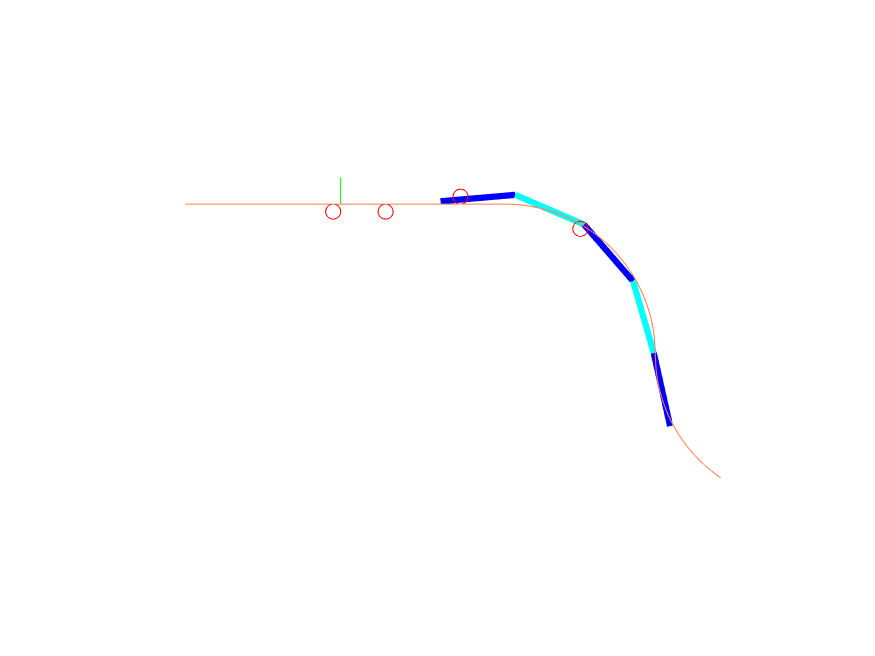
\includegraphics[trim=2cm 3cm 2cm 3cm, clip=true, totalheight=0.15\textheight]{figures/case-2-3/sim6.png}}
    
    \subfloat[$t = 120 s$]{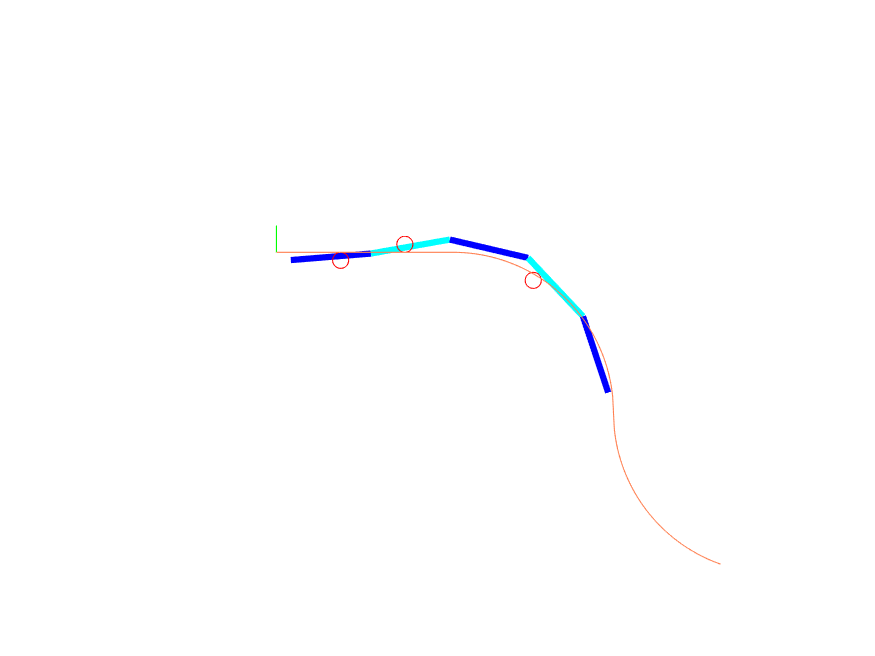
\includegraphics[trim=2cm 3cm 2cm 3cm, clip=true, totalheight=0.15\textheight]{figures/case-2-3/sim7.png}}
    \hfil
   
    \caption{Simulation demo - propulsion along path}
    \label{fig:case2-3}
\end{figure}


%---------------------------------------------------------------------------------------
%---------------------------------------------------------------------------------------
%---------------------------------------------------------------------------------------

